% Online Resource 1
\documentclass[pdflatex,sn-basic,Numbered]{sn-jnl}
\usepackage{graphicx,amsmath,amssymb,booktabs,array,tabularx,seqsplit}
\usepackage[title]{appendix}
\newcommand{\ttf}[1]{\texttt{\seqsplit{#1}}}
\setlength{\emergencystretch}{2em}
\raggedbottom
\AtBeginDocument{\hypersetup{
  pdftitle={Online Resource 1: Interaction-Aware Benchmarking of Exact-Gradient Signal and Finite-Shot Resolvability in a Four-Qubit Hybrid Quantum Neural Network},
  pdfauthor={Brandon Shen}
}}
\begin{document}

\title{Online Resource 1: Interaction-Aware Benchmarking of Exact-Gradient Signal and Finite-Shot Resolvability in a Four-Qubit Hybrid Quantum Neural Network}
\author*[1]{\fnm{Brandon} \sur{Shen} (ORCID: \href{https://orcid.org/0009-0002-3545-2106}{0009-0002-3545-2106})}\email{brandonshen123@gmail.com}
\affil*[1]{\orgname{Independent Researcher}, \orgaddress{\city{Belmont}, \state{California}, \postcode{94002}, \country{United States}}}
\maketitle

\begin{center}
\textbf{Supplementary Information for \textit{SN Computer Science}}
\end{center}

\section{Scope and frozen provenance}

This supplement reports the corrected centered H1--H4 family and the post-primary analyses frozen before manuscript revision. The machine-readable source of truth is indexed by \ttf{results/final\_submission\_v1/manifest.json} in the public repository, under the tag \ttf{submission-numerical-results-freeze-v1}. Historical outputs remain archived under \ttf{results/superseded/} and are not current primary results.

\section{Factor-coding correction and estimands}

The adopted factors are
\[
E_c=E-\tfrac12,\qquad L_c=L-\tfrac12,\qquad R_c=R-\tfrac12,
\]
with values $\{-1/2,+1/2\}$. Depth is $D_z=(D-3.2)/1.7204650534085253$, where 3.2 and 1.7204650534085253 are respectively the mean and population standard deviation of $D\in\{1,2,3,4,6\}$. Because $E_cL_cR_c$ remains in each applicable model, centered lower-order interactions average equally over the third binary factor. Direct-0/1 lower-order coefficients instead describe simple interactions at the third factor's reference level. The parameterizations yield identical fitted values, likelihood, residuals, and random effects; only the interpretation of lower-order coefficients changes. The correction was an implementation--interpretation correction rather than result-dependent model selection. H1 and H2 use $E_cL_c$, H3 uses $E_cR_c$ averaged over $L$, and H4 uses $L_cR_cD_z$.

\section{Corrected primary family and bootstrap}

\begin{table*}[t]
\centering
\footnotesize
\begin{tabularx}{\textwidth}{@{}l p{0.15\textwidth} r p{0.18\textwidth} r p{0.19\textwidth} X@{}}
\toprule
Hyp. & Estimand & Estimate & Wald 95\% CI & Holm $p$ & Bootstrap 95\% CI & Cross-method interpretation \\
\midrule
H1 & $E_cL_c$, exact & 0.004043 & [0.001924, 0.006162] & 0.000739 & [0.000473, 0.007535] & Model-based and bootstrap intervals exclude zero \\
H2 & $E_cL_c$, end-to-end & 0.014338 & [0.004255, 0.024422] & 0.015963 & [-0.016638, 0.043563] & Wald/Holm rejection; bootstrap includes zero \\
H3 & $E_cR_c$, end-to-end & -0.011615 & [-0.021697, -0.001534] & 0.047875 & [-0.030943, 0.010259] & Wald/Holm rejection; bootstrap includes zero \\
H4 & $L_cR_c\times$depth & -0.010179 & [-0.020688, 0.000331] & 0.057658 & [-0.026975, 0.006403] & Not rejected; remains unresolved \\
\bottomrule
\end{tabularx}
\caption{Corrected primary family. Wald intervals and Holm-adjusted $p$-values follow the primary model-based decision rule; the final interval column gives initialization-cluster percentile bootstrap results. H1 used 2,000 completed fits with zero failures, whereas H2--H4 used 443 completed nested-bootstrap fits. Bootstrap iterations are distinct from the 50 independent initialization clusters.}
\label{supp:tab:primary}
\end{table*}

For H2--H4, outer resampling selected complete initialization clusters and retained all configurations, depths, budgets, and matched parameters; within selected scientific cells, finite-shot replicates were resampled and SNR was recomputed before refitting. H1 resampled complete initialization clusters. Percentile intervals are reported without treating either Wald or bootstrap inference as universally preferable.

The frozen finite-shot production dataset used 30 independent gradient replicates per scientific cell and 50 independent top-level initialization clusters. The replicate pilot began at 30, evaluated candidate larger counts on prespecified representative cells, and did not satisfy its signed-mean and plug-in-SNR precision/stability criterion uniformly; the problem was most evident at shallow block counts. The already collected production dataset therefore retained 30, with no production recollection, making the sample sizes pilot-informed rather than pilot-calibrated.

The initialization-count pilot evaluated candidates in increments of 25 using the then-implemented H2--H4 mixed-model coefficients on the $\operatorname{asinh}(\mathrm{SNR}_{\mathrm{est}})$ response scale. At $N_{\mathrm{init}}=50$, the recorded 90th-percentile Wald 95\% CI half-widths were 0.1026212747780318 for $E{:}L$, 0.10253728880520716 for $E{:}R$, and 0.07250672321768473 for $L{:}R{:}\mathrm{depth}_z$, each below the configured 0.20 rule. That threshold was operational precision guidance on the transformed response scale, not a smallest effect of interest, equivalence margin, or scientific-importance claim. The pilot preceded the later centered-factor interpretation correction and did not evaluate H1.

The 443 H2--H4 draws comprised 8 previously validated draws plus three independently seeded 145-draw shards. All 443 fits completed successfully with zero failures. The documented target was at least 400 successful fits, with 1,000 preferred; execution stopped at the documented 145-draw-per-shard target, yielding 443. Checkpoint summaries at $n=40,100,200,400,$ and 443 retained the same qualitative conclusion: the relevant intervals included zero. These are completed bootstrap fits, not a sample size or a count of independent initialization clusters.

\section{Independent-seed H1 and depth weighting}

The independent-seed centered H1 estimate was $0.007726$ (Wald 95\% CI $[0.005592,0.009860]$); its 2,000-fit, zero-failure bootstrap interval was $[0.003402,0.011923]$. The direction was retained but magnitude remained uncertain.

\begin{table*}[t]
\centering\small
\resizebox{\textwidth}{!}{%
\begin{tabular}{crrrr}
\toprule
$D$ & Original estimate & Original 95\% CI & Independent-seed estimate & Independent-seed 95\% CI \\
\midrule
1 & -0.005251 & [-0.013708, 0.003206] & 0.001862 & [-0.006653, 0.010378] \\
2 & -0.003579 & [-0.009560, 0.002401] & 0.003120 & [-0.002901, 0.009141] \\
3 & 0.012588 & [0.007706, 0.017471] & 0.006250 & [0.001334, 0.011166] \\
4 & 0.004664 & [0.000435, 0.008892] & 0.007885 & [0.003627, 0.012143] \\
6 & 0.003446 & [-0.000007, 0.006898] & 0.010870 & [0.007393, 0.014346] \\
\midrule
Equal depth & 0.002374 & [-0.000164, 0.004911] & 0.005997 & [0.003443, 0.008552] \\
Observation/parameter weighted & 0.004043 & [0.001929, 0.006157] & 0.007726 & [0.005597, 0.009854] \\
\bottomrule
\end{tabular}}
\caption{Post-primary H1 depth contrasts and weighting summaries. Observation and matched-parameter weights are identical: 0.0625, 0.125, 0.1875, 0.25, and 0.375 at $D=1,2,3,4,6$. Intervals are unadjusted Wald 95\% intervals.}
\label{supp:tab:h1-depth}
\end{table*}

Original moderation tests were mixed-model $\chi^2(4)=22.844$, $p=0.000136$, and cluster-robust $\chi^2(4)=6.008$, $p=0.1985$. Independent-seed tests were $\chi^2(4)=7.563$, $p=0.1090$, and $\chi^2(4)=1.810$, $p=0.7706$. The original conclusion is covariance-sensitive; cross-seed magnitude differences have no clear depth localization under the frozen rule.

\begin{figure*}[t]\centering
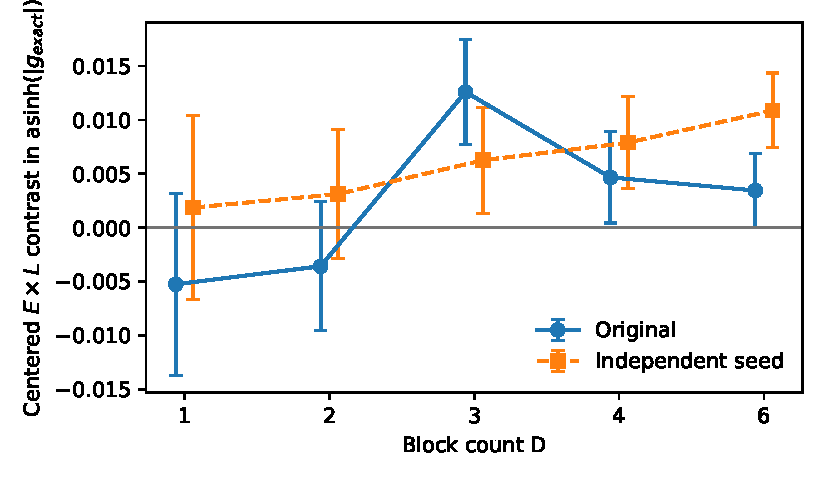
\includegraphics[width=.75\textwidth]{figures/fig13_h1_depth.pdf}
\caption{Post-primary centered H1 contrasts by block count. Bars are unadjusted Wald 95\% intervals; zero is the reference. Dataset identity is encoded by shape and line style, not color alone. No monotonic depth law is assumed.}
\end{figure*}

\begin{figure*}[t]\centering
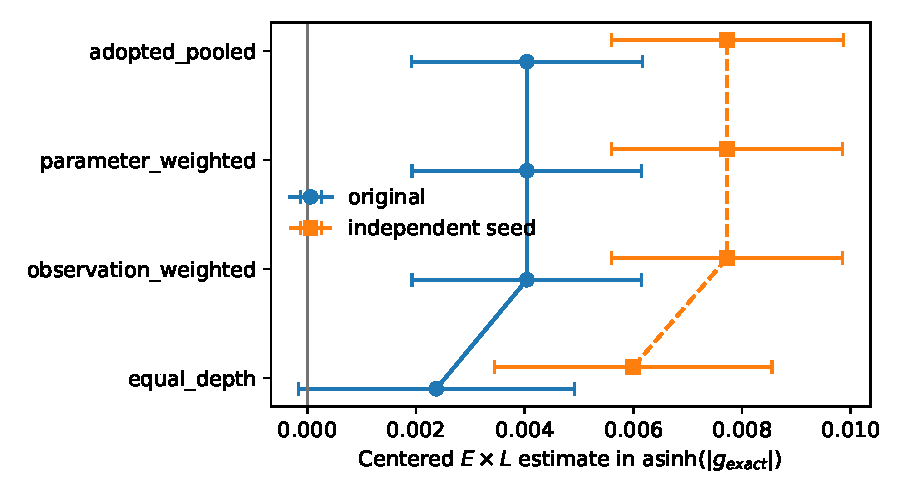
\includegraphics[width=.75\textwidth]{figures/fig14_h1_weighting.pdf}
\caption{Post-primary equal-depth, observation/matched-parameter, and adopted pooled H1 summaries. Bars are Wald 95\% intervals. Weightings answer different questions and were not selected by significance.}
\end{figure*}

\section{H3 post-primary explanatory analyses}

\begin{table*}[t]
\centering\small
\begin{tabular}{lrrr}
\toprule
Contrast or sensitivity & Estimate & Wald 95\% CI & Bootstrap 95\% CI \\
\midrule
End-to-end, $L=0$ & -0.000958 & [-0.015251, 0.013336] & [-0.030298, 0.024478] \\
End-to-end, $L=1$ & -0.022273 & [-0.036493, -0.008052] & [-0.048098, 0.007609] \\
End-to-end, L-average & -0.011615 & [-0.021697, -0.001534] & [-0.030943, 0.010259] \\
Active depths $D\ge3$, L-average & -0.014788 & [-0.024480, -0.005095] & Not planned \\
Conditional mode, L-average & 0.006978 & [-0.004745, 0.018701] & Not available \\
\bottomrule
\end{tabular}
\caption{Post-primary H3 explanatory and sensitivity results. Bootstrap intervals contain zero for both objective-specific contrasts and their average. Active-depth and conditional-mode rows are not substitutions for the primary model.}
\end{table*}

Depth-specific L-averaged estimates at $D=1,2,3,4,6$ were $0.006642$, $0.000696$, $-0.026492$, $-0.011553$, and $-0.011255$. Joint moderation did not reject with model-based ($p=0.545$) or cluster-robust ($p=0.721$) covariance. All 50 leave-one-initialization-out fits completed; all retained the negative averaged sign, 41 had raw $p<0.05$, and estimates ranged from $-0.014433$ to $-0.008562$. These diagnostics do not justify deletion. The frozen classification is a model-dependent directional signal, objective-specific under end-to-end mode.

\section{Conditional exact-gradient indices}

The frozen descriptive indices are
\[
J_{EL\mid R=0}=\frac{G_{EL}G_0}{G_EG_L},\qquad
J_{EL\mid R=1}=\frac{G_{ELR}G_R}{G_{ER}G_{LR}}.
\]
Unique exact-gradient parameter rows are pooled before the configuration-level RMS construction, so deeper depths receive more observation/parameter weight. The indices are conditional on $R$, not transformations of centered coefficients.

\begin{table}[t]\centering\small
\begin{tabular}{llrrr}
\toprule
Dataset & Estimand & Point & Median & Percentile 95\% CI \\
\midrule
Original & $J_{EL\mid R=0}$ & 1.241760 & 1.238674 & [1.082210, 1.414864] \\
Original & $J_{EL\mid R=1}$ & 1.126633 & 1.124329 & [0.991331, 1.285152] \\
Independent seed & $J_{EL\mid R=0}$ & 1.163219 & 1.160949 & [1.007100, 1.352596] \\
Independent seed & $J_{EL\mid R=1}$ & 1.242137 & 1.238157 & [1.049874, 1.449258] \\
\bottomrule
\end{tabular}
\caption{Conditional descriptive exact-gradient indices. Each initialization-cluster bootstrap completed 2,000 iterations with zero failures. Values above one are above the multiplicative no-interaction reference, not percentage improvements in optimization.}
\end{table}

\begin{figure}[t]\centering
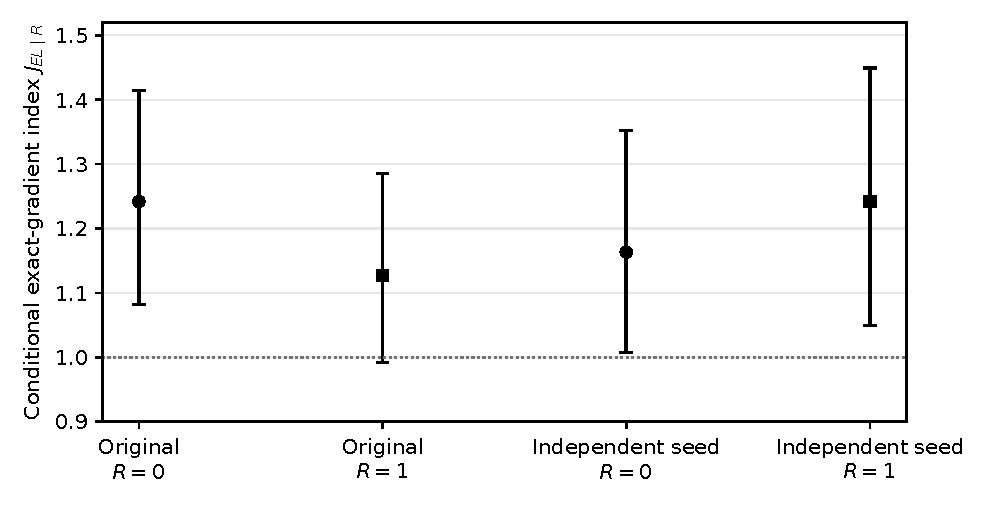
\includegraphics[width=.75\textwidth]{figures/fig12_j_conditional.pdf}
\caption{All four frozen conditional $J_{EL\mid R}$ estimates with percentile 95\% bootstrap intervals and reference line $J=1$. Marker shape identifies $R$ and line style identifies dataset. These are descriptive secondary ratios.}
\end{figure}

\section{Prepared-state metrics at initialization}

The frozen table contains 4,000 unique terminal-block states after exact-state duplication across shot budgets was removed. Fidelity and normalized-energy bounds, row uniqueness, energy spectral bounds, and fidelity--infidelity complementarity all passed. Original configuration--depth mean fidelity ranged approximately 0.0338--0.0817 and normalized energy 0.4631--0.5529; independent-seed ranges were 0.0322--0.0962 and 0.4561--0.5537. The ranges overlap strongly. Since $L$ changes evaluation rather than preparation, paired $L=0$/$L=1$ prepared-state summaries are identical. No significance test or causal gradient--task relationship is inferred.

\begin{table}[t]
\centering
\small
\begin{tabular}{lcc}
\toprule
Dataset & Cell-mean fidelity range & Cell-mean normalized-energy range \\
\midrule
Original & 0.0338--0.0817 & 0.4631--0.5529 \\
Independent seed & 0.0322--0.0962 & 0.4561--0.5537 \\
\bottomrule
\end{tabular}
\caption{Descriptive ranges across configuration--depth cell means for terminal-block prepared states at initialization. The overlapping ranges do not represent optimization trajectories or a test of gradient--task causality.}
\label{supp:tab:prepared-state-ranges}
\end{table}

\section{Measurement implementation and resource accounting}

Global infidelity is sampled directly from exact statevector overlap probability as one abstract overlap setting; no inverse target-state circuit, preparation gates, or physical cost is represented. TFIM energy uses a shared Z-basis multinomial setting for three $ZZ$ terms and a shared X-basis multinomial setting for four $X$ terms. End-to-end mode samples $D-1$ forward-feature Z jobs and re-encodes noisy features; conditional mode holds those features exact. Modes are not pooled.

All 320 resource rows conserve requested $B$ exactly, allocations are deterministic and nonnegative, and no production job has zero shots. All 1,833 zero-variance cells join to complete resource records. At $D=6$, conditional/global uses 48 jobs and end-to-end/local 61, a 27.08\% increase. The experiment matches total implemented simulator shots, not circuits, jobs, shots per circuit, physical gates, calibration, readout, hardware noise, or wall-clock time.

\section{Eligibility and zero-variance resource join}

Exactly zero replicate variance was restricted to $L=0$: 509 of 102,400 end-to-end and 1,324 of 102,400 conditional cells, with none under $L=1$. The primary finite-shot estimand therefore conditions on positive estimated variance. The resource join demonstrates that these exclusions do not reflect missing accounting records. They remain an objective-linked selection limitation.

\section{Historical correction and audit record}

Historical direct-0/1 coefficient tables and older pooled estimator-mode outputs are retained in explicitly superseded directories for auditability. They must not be read as current primary factorial conclusions. In particular, the former H3 value near $-0.000958$ is the end-to-end $E\times R$ simple interaction at $L=0$; it now appears as a post-primary explanatory contrast, not the centered H3 estimand. Historical `n=400' H1 bootstrap text is superseded by 2,000 completed fits. Historical H4 Holm $p=0.115$ is superseded by the corrected family value $0.057658$.

\section{Reproducibility index}

All frozen inputs, numerical outputs, figures, and verification reports are indexed by
\ttf{results/final\_submission\_v1/manifest.json} in the public repository
(\url{https://github.com/Brandon-Shen/few-qubit-qnn-snr}). The numerical state is tagged
\ttf{submission-numerical-results-freeze-v1}; the finalized manuscript commit is recorded in
\ttf{MANUSCRIPT\_COMMIT.txt}. The principal materials are grouped under:
\begin{itemize}
\item \ttf{results/primary\_corrected/} and \ttf{results/independent\_seed\_h1/} for corrected primary and independent-seed outputs;
\item \ttf{results/h1\_depth\_weighting/}, \ttf{results/h3\_centered\_robustness/}, and \ttf{results/jel\_conditional/} for post-primary analyses;
\item \ttf{results/task\_metrics/} and \ttf{results/resource\_accounting/} for descriptive task and measurement-resource outputs; and
\item \ttf{verification/} for plans, checksums, audit records, and machine-readable result reports.
\end{itemize}


\begin{appendices}
\section{Protocol and implementation interpretation}

\subsection{Factor-coding provenance}

The accessible protocol materials fixed the factorial interventions, hypotheses, transformations, model families, and Holm procedure but did not specify whether the binary predictors should be represented by direct 0/1 columns or centered $\{-1/2,+1/2\}$ columns. The original implementation fit the same full interaction model with direct 0/1 predictors and incorrectly interpreted lower-order pairwise coefficients as averages over the third factor. Re-expression with centered columns leaves fitted values, likelihood, residuals, and random effects unchanged while correcting the lower-order estimands. Historical direct-0/1 coefficients remain archived as reference-level simple interactions.

\subsection{Reset-per-block versus register-persisting semantics}

The protocol prose could be read in two ways. Under the adopted reset-per-block interpretation, every quantum block begins from $\lvert0000\rangle$, is measured independently, and passes only classical features to the next block. Under a register-persisting interpretation, the quantum state would continue across blocks. All code, gradients, shot accounting, and results in this study use the reset-per-block interpretation. Consequently, $D$ counts repeated quantum evaluations linked by classical re-encoding rather than layers of one continuously evolving quantum register. A register-persisting implementation would alter state preparation, entanglement propagation, derivative assembly, and measurement allocation and therefore constitutes a materially different experiment; the present results do not adjudicate that alternative.
\end{appendices}

\section{Remaining limitations}

Limitations include four qubits; one open-boundary TFIM task; reset-per-block architecture; one implementation per intervention; one initialization family; 50 top-level clusters per dataset; exact-state and abstract shot simulation; no hardware noise, readout, calibration, or optimization trajectories; prepared-state metrics only at initialization; $L$-linked finite-replicate zero-variance selection; depth weighting from parameter count; covariance-sensitive depth conclusions; H2/H3 procedure disagreement; H3 estimator-mode disagreement; weighting-dependent conditional J; inaccessible full protocol text as a factor-coding provenance limitation; and no matched physical-resource claim.

\end{document}
